% -*- coding: utf-8 -*-
\documentclass[11pt,a4paper]{article}
\usepackage[utf8]{inputenc}
\usepackage[T1]{fontenc}
\usepackage[spanish]{babel}
\usepackage{mathptmx} % Times-like, profesional
\usepackage{amsmath}  % Fórmulas matemáticas
\usepackage[margin=2.5cm,headheight=22pt]{geometry}
\usepackage{setspace}
\onehalfspacing

% Gráficos e imágenes (limitados a página para que no se salgan)
\usepackage{graphicx}
\usepackage{float}
\graphicspath{{./}{diagrams/}{docs/evidencias_jira/}}

% Encabezados al estilo TFM UNIR: autores (abrev.) + título corto + sección + página (ancho izquierdo acotado para no chocar con el número)
\usepackage{fancyhdr}
\pagestyle{fancy}
\fancyhf{}
\fancyhead[L]{\parbox[b]{0.82\headwidth}{\raggedright\sffamily\footnotesize Sandoval, Acevedo, Morales, Ríos --- Rehab. motriz asistida por CV --- \nouppercase{\rightmark}}}
\fancyhead[R]{\thepage}
\renewcommand{\headrulewidth}{0.4pt}
\renewcommand{\sectionmark}[1]{\markright{#1}}
\renewcommand{\subsectionmark}[1]{\markright{#1}}
\fancypagestyle{plain}{\fancyhf{}\fancyhead[L]{\parbox[b]{0.82\headwidth}{\raggedright\sffamily\footnotesize Sandoval, Acevedo, Morales, Ríos --- Rehab. motriz asistida por CV}}\fancyhead[R]{\thepage}\renewcommand{\headrulewidth}{0.4pt}}

% Tablas profesionales (booktabs)
\usepackage{booktabs}
\usepackage{array}
\usepackage{longtable}
\renewcommand{\arraystretch}{1.35}
\setlength{\arrayrulewidth}{0.5pt}

% Figuras y leyendas
\usepackage{caption}
\captionsetup{font=small,labelfont=bf,skip=8pt}
\captionsetup[figure]{position=below}
\captionsetup[table]{position=above}

% Hipervínculos y PDF
\usepackage[hidelinks]{hyperref}
\usepackage{url}

% Evitar viudas/huérfanas y saltos abruptos (estándar maestría)
\usepackage{needspace}
\raggedbottom
\widowpenalty=10000
\clubpenalty=10000
\sloppy

% Títulos de sección con estilo
\usepackage{titlesec}
\titleformat{\section}{\normalfont\sffamily\Large\bfseries}{\thesection.}{1em}{}
\titleformat{\subsection}{\normalfont\sffamily\large\bfseries}{\thesubsection}{1em}{}
\titleformat{\subsubsection}{\normalfont\sffamily\normalsize\bfseries}{\thesubsubsection}{1em}{}
\titlespacing*{\section}{0pt}{2.2ex plus .5ex}{1.2ex plus .3ex}
\titlespacing*{\subsection}{0pt}{1.8ex plus .4ex}{1ex plus .2ex}
\titlespacing*{\subsubsection}{0pt}{1.5ex plus .3ex}{0.8ex plus .2ex}

% Párrafos: sin sangría, espacio entre párrafos
\setlength{\parindent}{0pt}
\setlength{\parskip}{0.65em}

% ---------------------------------------------------------------------------
\title{Rehabilitación motriz asistida por visión por computadora}
\author{}
\date{}

\begin{document}

% ========== PORTADA (estándar TFM UNIR) ==========
\begin{titlepage}
\thispagestyle{empty}
\centering
\vspace*{1cm}
{\sffamily\fontsize{12}{16}\selectfont
Trabajo de innovación\\
\vspace{0.3cm}
Presentado por:\\
\vspace{0.4cm}
Cesar Francisco Sandoval González\\
Adelaid Lesdemyariet Acevedo Cardona\\
Armando Morales Carmona\\
José Rolando Ríos Cisneros\\
\vspace{0.5cm}
Ciudad: Madrid \quad Fecha: 27 de febrero de 2026\\
}
\vspace{1.2cm}
{\sffamily\fontsize{14}{18}\selectfont
Universidad Internacional de La Rioja (UNIR)\\
\vspace{0.25cm}
Escuela Superior de Ingeniería y Tecnología (ESIT)\\
\vspace{0.4cm}
Maestría en Inteligencia Artificial\\
}
\vspace{1.5cm}
\rule{\textwidth}{0.8pt}
\vspace{0.6cm}
{\sffamily\fontsize{15}{20}\selectfont\bfseries
Rehabilitación motriz asistida por visión por computadora\\
}
\vspace{0.3cm}
{\sffamily\fontsize{10}{13}\selectfont
Propuesta de trabajo de innovación\\
}
\vspace{0.4cm}
\rule{\textwidth}{0.8pt}
\vfill
\end{titlepage}

\clearpage
\pagenumbering{roman}
\setcounter{page}{1}

% ========== RESUMEN ==========
\phantomsection
\addcontentsline{toc}{section}{Resumen}
\begin{center}
{\sffamily\bfseries Resumen}
\end{center}
\vspace{0.5em}
\noindent La rehabilitación motriz tras un accidente cerebrovascular (ACV) enfrenta barreras de acceso y falta de supervisión objetiva en el domicilio. Este trabajo propone un prototipo de software basado en visión por computadora y aprendizaje automático que asiste la ejecución domiciliaria de ejercicios de hombro para pacientes post-ACV. El sistema utiliza una cámara web convencional, OpenCV y MediaPipe Pose para estimar la pose en 2D, calcula el ángulo de abducción del hombro y el conteo de repeticiones en tiempo real, y ofrece retroalimentación visual. El diseño se fundamenta en Design Thinking (empatía, reto HMW, estado del arte, selección de MVP) y en metodologías ágiles (Scrum y Lean Startup). La validación técnica se realizará mediante comparación con goniómetro y conteo humano, con criterios de éxito MAE $\leq$ 5° y precisión $\geq$ 95\,\%. Se concluye que la combinación de CV e IA de código abierto permite ofrecer supervisión objetiva accesible con hardware de consumo.

\vspace{0.8em}
\noindent Palabras clave: rehabilitación motriz, accidente cerebrovascular, visión por computadora, pose estimation, MediaPipe, tele-rehabilitación, Design Thinking, Scrum.

\clearpage
% ========== ABSTRACT ==========
\phantomsection
\addcontentsline{toc}{section}{Abstract}
\begin{center}
{\sffamily\bfseries Abstract}
\end{center}
\vspace{0.5em}
\noindent Motor rehabilitation after stroke faces barriers of access and lack of objective supervision at home. This work proposes a software prototype based on computer vision and machine learning to assist home-based shoulder exercises for post-stroke patients. The system uses a conventional webcam, OpenCV and MediaPipe Pose for 2D pose estimation, computes shoulder abduction angle and repetition count in real time, and provides visual feedback. The design is grounded in Design Thinking (empathy, HMW challenge, state of the art, MVP selection) and agile methodologies (Scrum and Lean Startup). Technical validation will be carried out by comparison with goniometer and human count, with success criteria MAE $\leq$ 5° and precision $\geq$ 95\,\%. It is concluded that the combination of open-source CV and AI can provide accessible objective supervision with consumer hardware.

\vspace{0.8em}
\noindent Keywords: motor rehabilitation, stroke, computer vision, pose estimation, MediaPipe, telerehabilitation, Design Thinking, Scrum.

\clearpage
% ========== ÍNDICE DE CONTENIDOS ==========
\tableofcontents
\clearpage
% ========== ÍNDICE DE TABLAS ==========
\listoftables
\clearpage
% ========== ÍNDICE DE FIGURAS ==========
\listoffigures
\clearpage
\pagenumbering{arabic}
\setcounter{page}{1}

% ========== 1. INTRODUCCIÓN ==========
\needspace{5\baselineskip}
\section{Introducción}

\subsection{Contexto y motivación}
El accidente cerebrovascular (ACV) constituye una de las principales causas de discapacidad motora adquirida a nivel mundial, con una incidencia que genera una carga significativa para los sistemas de salud y la calidad de vida de los individuos y sus familias (Organización Mundial de la Salud [OMS], 2017). En México es la quinta causa de muerte y la primera de discapacidad en adultos, situación que se refleja en diversas entidades federativas del país (Instituto Nacional de Estadística y Geografía [INEGI], 2021). Tras un ACV, hasta un 80\,\% de los supervivientes presenta hemiparesia o hemiplejía, requiriendo procesos prolongados de rehabilitación motriz para recuperar funcionalidad en las extremidades superiores; la movilidad del hombro es fundamental para las actividades de la vida diaria (Langhorne et al., 2011).

La rehabilitación tradicional, basada en terapia presencial y repetitiva, enfrenta barreras críticas de acceso: limitada disponibilidad de especialistas, altos costos asociados y dificultades geográficas para asistencia continua. Esta situación se agravó durante y después de la pandemia por COVID-19 y mostró la necesidad urgente de modelos complementarios de telerrehabilitación efectivos y escalables (Laver et al., 2020). La Inteligencia Artificial (IA) emerge como catalizador de innovación en salud, con herramientas para monitorización objetiva, personalización de terapias y extensión del cuidado más allá del entorno clínico (Esteva et al., 2019).

\subsection{Planteamiento del problema}
Existe una brecha crítica entre la necesidad de rehabilitación motriz intensiva y repetitiva post-ACV y la capacidad del sistema de salud para proporcionar un acceso continuo, supervisado y asequible a dichos servicios. Los pacientes que realizan ejercicios en domicilio carecen de retroalimentación objetiva en tiempo real sobre la calidad de su movimiento, lo que puede conducir a una ejecución incorrecta, compensaciones musculares indeseadas, baja adherencia al tratamiento y, en última instancia, una recuperación funcional subóptima.

Si bien existen soluciones tecnológicas en el mercado (sistemas basados en Kinect, sensores inerciales o robótica), estas suelen presentar barreras de costo, complejidad técnica o necesidad de hardware especializado, limitando su adopción masiva en el ámbito domiciliario. De ahí la necesidad de una solución accesible, de bajo costo y fácil de usar que, con hardware convencional, permita supervisar, evaluar y guiar ejercicios de rehabilitación de forma autónoma.

\subsection{Justificación e innovación}
Esta propuesta se justifica por su potencial para generar un impacto tangible en un problema de salud pública, alineándose con los Objetivos de Desarrollo Sostenible (ODS), particularmente con el ODS 3 (Salud y bienestar). La innovación no radica en la creación de un nuevo algoritmo de estimación de pose, sino en la aplicación integrada, simplificada y centrada en el usuario de tecnologías de visión por computadora (CV) e IA de código abierto para resolver un problema clínico específico.

El valor agregado reside en su viabilidad y accesibilidad: utiliza una cámara web estándar y librerías de software libre (OpenCV, MediaPipe), eliminando la dependencia de hardware costoso. Su novedad está en el diseño de un sistema integral que, partiendo de la detección de pose, automatiza la evaluación cuantitativa (ángulos, repeticiones) y proporciona retroalimentación correctiva inmediata, emulando funciones clave del terapeuta y empoderando al paciente en su proceso de recuperación domiciliaria. La solución plantea además potencial como herramienta tecnológica escalable en el ámbito de salud digital, alineada con tendencias de telemedicina y rehabilitación remota (National Institute of Neurological Disorders and Stroke [NINDS], 2020). La contribución de este trabajo es demostrar que la combinación de visión por computadora e IA en código abierto puede ofrecer supervisión objetiva en rehabilitación domiciliaria con hardware de consumo, abriendo una vía de uso de la IA distinta a las soluciones costosas o sin retroalimentación automática.

\subsection{Alcance}
El proyecto se desarrollará en un plazo de 16 semanas, dentro del marco del Seminario de Innovación en IA de UNIR. El alcance del Producto Mínimo Viable (MVP) se delimita específicamente a:
\begin{itemize}
  \item Población: personas con secuelas motoras en miembro superior tras un ACV (simulada inicialmente con sujetos sanos para pruebas de concepto);
  \item Ejercicio: abducción/aducción de hombro en el plano frontal (elevación lateral del brazo), por ser un movimiento fundamental y evaluable;
  \item Tecnología: visión por computadora 2D, sin uso de sensores de profundidad ni hardware adicional;
  \item Objetivo: validar la precisión técnica del sistema en medición angular y conteo, no la efectividad clínica a largo plazo (lo cual requeriría un estudio posterior).
\end{itemize}
El éxito de la validación se medirá mediante criterios explícitos y verificables: Error Absoluto Medio (MAE) $\leq$ 5° en la medición angular frente a goniómetro como referente estándar, y precisión $\geq$ 95\,\% en el conteo de repeticiones respecto al conteo realizado por un evaluador humano. Las definiciones formales de estas métricas se detallan en la Sección 6 (Validación). Estos indicadores, vinculados directamente al alcance del MVP, permiten verificar el cumplimiento de los criterios de forma reproducible.

\subsection{Estructura del documento}
El cuerpo del documento comprende siete secciones numeradas (1--7), seguidas de Anexos y Referencias. La secuencia es: Sección 1, Introducción; Sección 2, Objetivos; Sección 3, Desarrollo conceptual (Design Thinking); Sección 4, Metodología (Scrum y Lean); Sección 5, Implementación; Sección 6, Validación y diseño experimental; Sección 7, Conclusiones y trabajo futuro; a continuación los Anexos y las Referencias. Para esta entrega, el documento se presenta y evalúa hasta la Sección 5 (Metodología); las secciones 6 y 7 y los Anexos forman parte de la estructura completa pero quedan fuera del alcance de la evaluación actual. El orden sigue la lógica: qué se busca (objetivos), por qué y para quién (conceptual), cómo se ejecutará (metodología e implementación) y cómo se demostrará el logro (validación). Los criterios de éxito (MAE $\leq$ 5°, precisión $\geq$ 95\,\%) se validan en la Sección 6 mediante el protocolo experimental. La validación del MVP se contrastará frente al goniómetro como estándar clínico de medición angular y al conteo humano como referente de conteo de repeticiones.

\clearpage
\needspace{5\baselineskip}
\section{Objetivos}

\subsection{Objetivo general}
Desarrollar un prototipo de software basado en visión por computadora que asista la ejecución domiciliaria de ejercicios de rehabilitación de hombro para pacientes post-ACV, verificando su precisión técnica mediante la comparación con un goniómetro y conteo humano para lograr un Error Absoluto Medio (MAE) $\leq$ 5° y una precisión $\geq$ 95\,\%.

\subsection{Objetivos específicos}
Para lograr el objetivo general, se establecen los siguientes objetivos específicos, con evidencia esperada asociada:

\begin{itemize}
  \item Implementar un módulo de estimación de pose humana en 2D que detecte de forma estable las coordenadas de puntos anatómicos clave desde el flujo de video de una cámara web con MediaPipe Pose.
  \begin{itemize}
    \item \textit{Evidencia esperada:} módulo funcional integrado que procesa video en tiempo real.
  \end{itemize}
  \item Desarrollar algoritmos de análisis cinemático que calculen en tiempo real el ángulo de abducción del hombro (geometría vectorial cadera--hombro--codo) e identifiquen ciclos de movimiento.
  \begin{itemize}
    \item \textit{Evidencia esperada:} funciones probadas que devuelven ángulo en grados y estado del ciclo por frame.
  \end{itemize}
  \item Integrar un sistema de interfaz y retroalimentación que muestre video anotado, ángulo actual, contador de repeticiones y mensajes correctivos.
  \begin{itemize}
    \item \textit{Evidencia esperada:} ventana gráfica operativa con los cuatro elementos integrados.
  \end{itemize}
  \item Validar el rendimiento del prototipo comparando sus métricas contra un goniómetro y conteo humano.
  \begin{itemize}
    \item \textit{Evidencia esperada:} informe con valores de MAE, precisión y conclusiones sobre el cumplimiento de los criterios.
  \end{itemize}
  \item Documentar el proceso, el código y los resultados en un repositorio Git con un informe de validación.
  \begin{itemize}
    \item \textit{Evidencia esperada:} repositorio con README, código comentado e informe de validación.
  \end{itemize}
\end{itemize}

\clearpage
\needspace{5\baselineskip}
\section{Desarrollo conceptual (Design Thinking)}

El capítulo aplica Design Thinking en seis etapas para definir la solución, anclada en las necesidades del usuario, el estado del arte y la viabilidad técnica.

\subsection{Empatizar}
La etapa de empatía se centró en comprender en profundidad las experiencias, frustraciones y aspiraciones de los dos usuarios principales: el paciente post-ACV y el terapeuta rehabilitador.

Método y análisis. La búsqueda bibliográfica se realizó en las bases de datos PubMed, IEEE Xplore y Scopus, combinando términos MeSH y palabras clave: (\textit{stroke rehabilitation} OR \textit{post-stroke}) AND (\textit{computer vision} OR \textit{pose estimation} OR \textit{MediaPipe}) AND (\textit{home-based} OR \textit{telerehabilitation}). El período se limitó a publicaciones entre 2020 y 2026 para favorecer la actualidad, con énfasis en 2024--2026 en inteligencia artificial aplicada a la rehabilitación. En paralelo se revisaron guías y síntesis clínicas (OMS, Langhorne et al., Laver et al.) y se categorizaron necesidades en pains y gains por perfil de usuario, triangulando literatura clínica y reportes tecnológicos (Debnath et al., 2021; Saposnik et al., 2016).

Para complementar el análisis documental y anclar los pains/gains en evidencia obtenida con participantes (datos primarios publicados), se analizó en profundidad el estudio de factibilidad de Unger et al. (2025), publicado en \textit{Frontiers in Medicine}. Los autores reclutaron a 20 personas con ictus y deterioro leve a moderado del miembro superior, que ejecutaron una tarea funcional de beber registrada con cámara web de consumo y otras cámaras, con un sistema de captura óptica de movimiento como referencia cinemática; las secuencias fueron etiquetadas por terapeutas respecto a la presencia de compensaciones, se extrajeron poses con MediaPipe y se entrenaron modelos de aprendizaje profundo sobre los keypoints. Ese diseño aporta hallazgos cuantitativos alineados con las necesidades detectadas en la literatura secundaria.

Para el paciente: dolor --- acceso limitado y costoso a terapia presencial continua, desmotivación y falta de adherencia por monotonía y ausencia de retroalimentación inmediata, incertidumbre sobre la corrección de los ejercicios domiciliarios; ganancia --- autonomía para ejercitarse en casa, guía y confirmación del movimiento, progreso tangible y sistema accesible sin alta inversión. Para el terapeuta: dolor --- imposibilidad de supervisar de forma objetiva y continua la rehabilitación domiciliaria, carga administrativa alta, dificultad para cuantificar rango de movimiento o repeticiones efectivas; ganancia --- datos objetivos y automatizados, ajuste del tratamiento basado en evidencia cuantitativa, optimización del tiempo de consulta. Estudios recientes indican que tecnologías como la realidad virtual pueden aumentar la adherencia del paciente, aunque no siempre se traducen en mejoras clínicas significativas superiores a la terapia convencional (Saposnik et al., 2016).

\begin{table}[htbp]
\caption{Resumen de hallazgos de la etapa Empatizar.}
\label{tab:empatizar}
\small
\centering
\renewcommand{\arraystretch}{1.35}
\begin{tabular}{@{}p{2.5cm}p{4.7cm}p{4.7cm}@{}}
\toprule
Usuario / foco & Dolor & Ganancia \\
\midrule
Paciente post-ACV & Acceso limitado a terapia; desmotivación y baja adherencia; incertidumbre sobre la corrección del ejercicio domiciliario. & Autonomía en casa; guía y confirmación del movimiento; progreso tangible; sistema accesible y de bajo costo. \\
\addlinespace
Terapeuta & Imposibilidad de supervisar y cuantificar el trabajo domiciliario; carga administrativa. & Datos objetivos automatizados; ajuste del tratamiento con evidencia; optimización del tiempo de consulta. \\
\addlinespace
Evidencia empírica (Unger et al., 2025) --- paciente & La detección entre personas no generalizó bien: con keypoints crudos de MediaPipe, la precisión interindividual rondó el 50\,\%; la clasificación dentro de la misma persona superó típicamente el 90\,\%. & Refuerza la necesidad de enfoques personalizables o adaptables y de características más informativas que los keypoints crudos. \\
\addlinespace
Evidencia empírica (Unger et al., 2025) --- terapeuta / supervisión & Las etiquetas clínicas y el uso de visión por computadora aún dejan una tarea difícil: los modelos interpersonales con señal MediaPipe sola quedaron en torno al 50\,\% de acierto hasta incorporar ingeniería de características o datos de referencia más ricos (OMC). & Subraya la dificultad de la supervisión automatizada y el valor de sistemas bien calibrados y trazables en domicilio. \\
\bottomrule
\end{tabular}\\
\renewcommand{\arraystretch}{1.35}
\vspace{4pt}
\raggedright\footnotesize Fuente: elaboración propia a partir de OMS, Langhorne et al., Laver et al., Debnath et al. (2021), Saposnik et al. (2016) y Unger et al. (2025).
\end{table}
\vspace{0.6em}

Esta comprensión estableció la base humana del proyecto: la necesidad de un puente tecnológico confiable entre la clínica y el hogar.

Además de la evidencia publicada, cabe la posibilidad de un refuerzo con fuente primaria local (entrevista semiestructurada a un experto en rehabilitación u observación estructurada de sesión), siguiendo guion o ficha, registro y síntesis; la decisión y el registro metodológico se recogen en el Anexo~C.

Trazabilidad narrativa. Los hallazgos de la Tabla~\ref{tab:empatizar} derivaron en el reto HMW (Definir); los criterios de éxito se alinearon con las ganancias identificadas (accesibilidad, precisión, retroalimentación, trazabilidad); la selección del prototipo (Idea C) se sustentó en esos criterios mediante la matriz ponderada. El flujo hallazgos -- reto -- criterios -- decisiones del MVP queda así trazado (Figura~\ref{fig:flujo}).

\vspace{1.2em}
\begin{figure}[htbp]
\centering
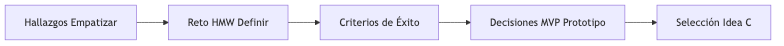
\includegraphics[width=0.85\linewidth,height=0.48\textheight,keepaspectratio]{flujo_design_thinking.png}
\caption{Trazabilidad Empatizar--Definir--Criterios--MVP.}
\label{fig:flujo}
\raggedright\footnotesize Fuente: Elaboración propia.
\end{figure}
\vspace{0.8em}

\subsection{Definir (HMW y criterios de éxito)}
Sintetizando los hallazgos de la empatía, se formuló el siguiente reto de diseño, estructurado como una pregunta ``How Might We?'' (¿Cómo podríamos?):

\begin{quote}
\small ¿Cómo podría lograrse que los pacientes post-ACV dispongan de una herramienta de rehabilitación motriz domiciliaria tan accesible como una cámara web, pero con supervisión y retroalimentación objetiva comparable a la guía inicial de un terapeuta, de modo que mejoren la confianza, la adherencia y la calidad del ejercicio?
\end{quote}

A partir de este reto se derivaron los Criterios de Éxito iniciales para la solución:
\begin{enumerate}
  \item Accesibilidad económica: costo de implementación cercano a cero para el usuario final (hardware de consumo estándar).
  \item Precisión técnica: capacidad de medir ángulos articulares con un error aceptable frente a instrumentos estándar (goniómetro).
  \item Retroalimentación en tiempo real: generación de guías visuales o auditivas inmediatas durante la ejecución del ejercicio.
  \item Usabilidad: interfaz intuitiva que no requiera capacitación extensa.
  \item Trazabilidad: registro automático de métricas (repeticiones, ángulos máximos) para seguimiento del progreso.
\end{enumerate}
Estos criterios se operacionalizarán en el diseño experimental (Sección 6) mediante MAE $\leq$ 5°, precisión $\geq$ 95\,\% y latencia $<$ 150\,ms.

\subsection{Investigación de antecedentes (estado del arte)}
Se revisaron las soluciones existentes en rehabilitación asistida por tecnología (Debnath et al., 2021). La Tabla~\ref{tab:estadoarte} compara distintas aproximaciones según integración con el paciente y aplicabilidad clínica, apoyada en la literatura (Basteris et al., 2014; Debnath et al., 2021; Saposnik et al., 2016).

\begin{table}[htbp]
\caption{Análisis comparativo del estado del arte en rehabilitación asistida.}
\label{tab:estadoarte}
\small
\centering
\renewcommand{\arraystretch}{1.45}
\begin{tabular}{@{}p{2.4cm}p{2.5cm}p{2.2cm}p{2.5cm}p{2.9cm}@{}}
\toprule
Categoría & Descripción & Ventajas & Desventajas & Posicionamiento \\
\midrule
Terapia manual convencional & Supervisión presencial por fisioterapeuta. & Estándar de oro, evaluación integral. & Coste elevado, acceso limitado. & Complementar la terapia con métricas objetivas en domicilio. \\
\addlinespace
Robótica y exoesqueléticos & Sistemas que asisten el movimiento (ej. Armeo Power). & Alta precisión, asistencia física. & Costo prohibitivo, confinados a clínicas. & Alternativa no robótica y de bajo costo. \\
\addlinespace
Realidad virtual & Entornos inmersivos (ej. Oculus Quest, VITALIS). & Alta motivación y adherencia. & Costo moderado-alto, no siempre superioridad clínica. & Precisión de medición y corrección del movimiento real. \\
\addlinespace
Software clínico & Gestión y prescripción (SPRY, WebPT). & Excelente para gestión. & Enfocados en administración, no en evaluación en tiempo real. & Análisis automático de movimiento como módulo complementario. \\
\addlinespace
Apps móviles instructivas & Videos y recordatorios. & Muy accesibles, bajo costo. & Sin retroalimentación objetiva. & Análisis y retroalimentación automatizada en tiempo real. \\
\bottomrule
\end{tabular}\\
\renewcommand{\arraystretch}{1.35}
\vspace{4pt}
\raggedright\footnotesize Fuente: Basteris et al. (2014); Debnath et al. (2021); Saposnik et al. (2016).
\end{table}
\vspace{0.6em}

Conclusión del análisis. Hay una brecha entre soluciones de alta tecnología (robótica, VR), costosas y complejas, y otras muy accesibles (apps, videos) pero sin supervisión inteligente. La propuesta apunta a ese hueco: una ``supervisión inteligente accesible'' que permita análisis automático del movimiento con hardware estándar. La solución aquí seleccionada combina cámara 2D, procesamiento local y criterios de validación cuantitativos explícitos (MAE $\leq$ 5°, precisión $\geq$ 95\,\%) en un único prototipo orientado al ámbito domiciliario.

En el ámbito específico de la \textbf{estimación de pose para rehabilitación}, Shukla y Rathore (2025) presentan PoseRx, un modelo basado en transformadores (TokenPose) con error medio absoluto angular (MAE) de 5,4° y error de localización 2D de 5,9 píxeles, con alta robustez ante oclusiones (véase desglose en el Anexo~D). Ese orden de magnitud sirve como \textbf{baseline técnico} para contextualizar el criterio de éxito del presente MVP (MAE $\leq$ 5°): si un modelo complejo alcanza 5,4°, un sistema bien calibrado con MediaPipe en hardware de consumo puede aspirar a un MAE no superior a 5° en el protocolo de validación descrito en la Sección~6.

\subsection{Idear}
Se generaron múltiples alternativas evaluando distintas combinaciones de tecnología y entrega. Se consideraron tres opciones que cubren los escenarios más plausibles (dispositivo móvil, procesamiento en nube, procesamiento local en escritorio) para comparar accesibilidad, privacidad y viabilidad técnica.

\begin{itemize}
  \item Idea A --- Teléfono inteligente como sensor y pantalla: app móvil que use la cámara del teléfono para capturar el movimiento y muestre la retroalimentación en la misma pantalla.
  \item Idea B --- Sistema web con procesamiento en la nube: aplicación web con streaming de video; el procesamiento de visión por computadora se realizaría en un servidor remoto.
  \item Idea C --- Software de escritorio con procesamiento local (propuesta actual): aplicación para computadora personal (Windows/macOS/Linux) que utilice cámara web externa y procese toda la información localmente.
\end{itemize}

\subsection{Prototipar}
Se seleccionó la Idea C para prototipar. El MVP será un script en Python ejecutable, con interfaz gráfica simple, que cumpla el flujo core: (1) Entrada: captura de video en tiempo real desde cámara web USB estándar (720p o superior). (2) Procesamiento: pipeline con OpenCV y MediaPipe Pose (modelo \texttt{pose\_landmarker\_lite} por defecto; opcional \texttt{pose\_landmarker\_full}). (3) Lógica: cálculo del ángulo de abducción del hombro en tiempo real con geometría vectorial (landmarks cadera, hombro, codo); detección de repeticiones mediante máquina de estados con umbrales angulares. (4) Salida: ventana con video y esqueleto superpuesto, valor del ángulo, contador de repeticiones y mensajes de texto (ej. ``Extienda más el brazo'', ``Repetición válida''). La interfaz se estructura en tres zonas: área central de video con esqueleto; panel de métricas (ángulo y contador); barra inferior de mensajes. La Figura~\ref{fig:flujo-prototipo} muestra el flujo de uso del prototipo MVP desde la perspectiva del usuario. El diagrama del pipeline de componentes se describe en la Sección~5 (Implementación).

\vspace{1em}
\begin{figure}[htbp]
\centering
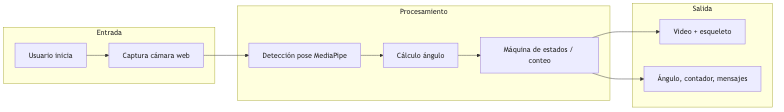
\includegraphics[width=0.9\linewidth,height=0.35\textheight,keepaspectratio]{flujo_prototipo_uso.png}
\caption{Flujo de uso del prototipo MVP: entrada (captura), procesamiento (pose, ángulo, conteo) y salida (video anotado, métricas y mensajes).}
\label{fig:flujo-prototipo}
\raggedright\footnotesize Fuente: Elaboración propia.
\end{figure}
\vspace{0.6em}

\subsection{Selección de prototipo}
Para justificar formalmente la elección de la Idea C se utilizó una matriz de selección ponderada con criterios alineados al marco MELDS (Tabla~\ref{tab:melds}). La Idea C (software de escritorio) obtuvo la puntuación más alta en privacidad, accesibilidad y viabilidad técnica (puntuación total ponderada 9,15), criterios centrales para el MVP en 16 semanas. Resuelve el problema de supervisión automatizada accesible de forma directa y con menor riesgo técnico.

\begin{table}[htbp]
\caption{Matriz de selección y evaluación de ideas (MELDS).}
\label{tab:melds}
\small
\centering
\renewcommand{\arraystretch}{1.5}
\begin{tabular}{@{}p{3cm}c p{2.5cm} p{2.5cm} p{2.5cm} c@{}}
\toprule
Criterio & Peso & Idea A & Idea B & Idea C & \\
\midrule
Viabilidad técnica & 25\,\% & Alta (8) & Media-baja (4) & Alta (9) & \\
Costo/Accesibilidad & 25\,\% & Alta (9) & Media (6) & Muy alta (10) & \\
Precisión y control & 20\,\% & Media (6) & Media-alta (7) & Alta (9) & \\
Privacidad y ética & 20\,\% & Alta (8) & Baja (3) & Muy alta (10) & \\
Potencial integración & 10\,\% & Media (5) & Alta (8) & Media-alta (7) & \\
\midrule
Puntaje total ponderado & 100\,\% & 7,45 & 5,45 & 9,15 & \\
\bottomrule
\end{tabular}\\
\renewcommand{\arraystretch}{1.35}
\vspace{4pt}
\raggedright\footnotesize Fuente: Elaboración propia (marco MELDS).
\end{table}
\vspace{0.6em}

\clearpage
\needspace{5\baselineskip}
\section{Metodología: Scrum y Lean}

Este capítulo detalla el marco de trabajo ágil y la filosofía de desarrollo adoptados en el proyecto. La combinación de Scrum y Lean Startup (Ries, 2011) proporciona una estructura para organizar el trabajo en equipo, priorizar el valor, gestionar la incertidumbre y asegurar que el desarrollo del prototipo se mantenga enfocado, iterativo y basado en evidencia.

\subsection{Roles, artefactos y eventos}
El proyecto adopta Scrum con responsabilidades claras. Roles: Product Owner (Cesar Francisco Sandoval González): maximizar el valor del producto y gestionar el backlog. Scrum Master (Adelaid Lesdemyariet Acevedo Cardona): facilitar el proceso y eliminar impedimentos. Equipo de desarrollo (Armando Morales Carmona y José Rolando Ríos Cisneros): analizar, diseñar, desarrollar, probar y documentar el incremento en cada sprint. Artefactos: Product Backlog (lista priorizada), Sprint Backlog (subconjunto del sprint), Incremento (suma de elementos completados). Eventos: Sprint Planning (inicio de cada sprint semanal), Daily Stand-up (15 min), Sprint Review (presentación del incremento), Sprint Retrospective (mejora de proceso).

\subsection{Backlog inicial, estimación y cadencia}
El backlog reúne historias de usuario y tareas técnicas estimadas con puntos de historia (escala de Fibonacci: 1, 2, 3, 5, 8). Criterio de puntos: 1 = trivial; 2 = simple; 3 = moderada; 5 = compleja; 8 = muy compleja o alta incertidumbre. Sprints de una semana; los diez primeros sprints cubren el núcleo del backlog (Tabla~\ref{tab:backlog}), enmarcados en un calendario total de 16 semanas del seminario (véase Sección~5).

El \textbf{equipo de desarrollo} (Armando Morales Carmona y José Rolando Ríos Cisneros) tiene una dedicación estimada de 20\,h semanales cada uno, es decir, \textbf{40\,h de capacidad por sprint} dedicadas a análisis, implementación y pruebas. El Product Owner y el Scrum Master participan en planificación, revisión y gestión del backlog con criterios de disponibilidad propios del proyecto, sin contabilizarse en esas 40\,h. Con la complejidad inicial del backlog, se estima una \textbf{velocidad inicial de 8--10 puntos de historia por sprint}, que se ajustará según la velocidad observada ($V_s = \sum_{j \in \mathcal{C}_s} p_j$ puntos completados en el sprint $s$). La Tabla~\ref{tab:backlog} presenta el backlog priorizado con criterios de aceptación verificables.

\begin{table}[htbp]
\caption{Backlog del producto con criterios de aceptación por historia.}
\label{tab:backlog}
\small
\centering
\renewcommand{\arraystretch}{1.45}
\begin{tabular}{@{}p{0.75cm}p{2.7cm}p{5.8cm}p{0.5cm}p{0.6cm}@{}}
\toprule
ID & Historia / Tarea & Criterios de aceptación & Pts & Spr. \\
\midrule
US-01 & Configuración del entorno & venv creado; requirements.txt con opencv-python, mediapipe, numpy; script de prueba que importa librerías; proyecto en Git con /src, /docs, /data. & 1 & 1 \\
\addlinespace
US-02 & Captura de video en tiempo real & Captura con OpenCV; ventana con video en vivo; cierre correcto; resolución 720p o superior. & 2 & 1 \\
\addlinespace
US-03 & Visualización del esqueleto & MediaPipe Pose integrado; dibujo de landmarks y conexiones; hombro, codo y cadera visibles; integrado con US-02. & 3 & 2 \\
\addlinespace
US-04 & Cálculo y visualización de ángulo & Ángulo de abducción (cadera--hombro--codo); valor en grados visible; actualización frame a frame; código documentado. & 5 & 3 \\
\addlinespace
US-05 & Conteo automático de repeticiones & Máquina de estados (subida/bajada); umbrales configurables (60°); contador visible; sin falsos positivos evidentes. & 5 & 4 \\
\addlinespace
US-06 & Retroalimentación de corrección & Mensajes según reglas; criterios por umbrales; mensajes en zona dedicada; integración con conteo. & 8 & 5 \\
\addlinespace
T-07 & Diseño del protocolo de validación & Documento con hipótesis, métricas y criterios; fases: reclutamiento, configuración, ejecución, análisis; materiales y revisión. & 3 & 7 \\
\addlinespace
T-08 & Pruebas de validación y datos & $\geq$5 sujetos; consentimiento firmado; 3$\times$10 repeticiones con goniómetro y grabación; logs CSV y backup. & 8 & 8--9 \\
\addlinespace
T-09 & Análisis y gráficos & Script que calcula MAE, precisión y latencia; gráficos y tablas; informe con resultados y limitaciones. & 5 & 10 \\
\addlinespace
US-10 & Exportación de reportes & Exportación a CSV; opción PDF si hay tiempo; documentado en README. & 5 & 6 \\
\bottomrule
\end{tabular}\\
\renewcommand{\arraystretch}{1.35}
\vspace{4pt}
\raggedright\footnotesize Fuente: Elaboración propia (Scrum/Lean).
\end{table}
\vspace{0.6em}

Cada sprint entrega un incremento verificable. Los \textbf{objetivos explícitos por sprint} (alineados con la columna \textit{Spr.} de la Tabla~\ref{tab:backlog}) son:
\begin{enumerate}\setlength{\itemsep}{0.35em}
  \item \textbf{Sprint 1 (semana 1):} configurar el entorno de desarrollo y lograr captura de video básica con OpenCV (US-01, US-02).
  \item \textbf{Sprint 2 (semana 2):} integrar MediaPipe Pose y visualizar el esqueleto en tiempo real (US-03).
  \item \textbf{Sprint 3 (semana 3):} implementar y mostrar en pantalla el cálculo del ángulo de abducción del hombro (US-04).
  \item \textbf{Sprint 4 (semana 4):} desarrollar la máquina de estados y el contador de repeticiones (US-05).
  \item \textbf{Sprint 5 (semana 5):} integrar la retroalimentación visual y textual basada en umbrales (US-06).
  \item \textbf{Sprint 6 (semana 6):} estabilizar el prototipo e incorporar la exportación de datos a CSV (US-10).
  \item \textbf{Sprint 7 (semana 7):} diseñar y documentar el protocolo de validación experimental (T-07).
  \item \textbf{Sprints 8--9 (semanas 8--9):} ejecutar las pruebas de validación con sujetos sanos y registrar los datos (T-08).
  \item \textbf{Sprint 10 (semana 10):} analizar los datos, generar gráficos (MAE, precisión) y redactar el informe de validación (T-09).
\end{enumerate}

Dependencias entre ítems: US-03 requiere US-02; US-04 requiere US-03; US-05 requiere US-04; US-06 requiere US-05; US-10 requiere US-06; T-07 es independiente de las historias de implementación; T-08 requiere T-07; T-09 requiere T-08.

Las \textbf{semanas 11--16} del calendario del seminario se destinan a consolidación, ajustes finales, documentación académica y cierre de entregas (véase Sección~5), sin duplicar la numeración de sprints anteriores.

\subsection{Definiciones de Ready/Done}
Definición de listo (DoR): la historia está lista para el sprint cuando está claramente descrita, tiene criterios de aceptación conocidos, dependencias resueltas, estimada por el equipo y es completable en un sprint. Definición de hecho (DoD): el código está escrito y documentado, la funcionalidad está integrada, se han ejecutado pruebas unitarias e de integración con resultados satisfactorios, hay peer review y la documentación está actualizada.

\subsection{Principios Lean, ciclo operativo y métricas}
La filosofía Lean se integra en cinco etapas por sprint: (1) Idear --- refinamiento del backlog e hipótesis; (2) Construir --- desarrollo hasta cumplir DoD; (3) Medir --- velocidad, bug rate post-DoD, valor cualitativo del Product Owner; (4) Aprender --- validated learning y Kaizen en retrospectiva; (5) Decidir --- continuar o ajustar según umbrales (velocidad, bug rate, valor del incremento). La velocidad del equipo se define como la suma de puntos de historia completados en el sprint: $V_s = \sum_{j \in \mathcal{C}_s} p_j$, donde $\mathcal{C}_s$ es el conjunto de ítems completados en el sprint $s$ y $p_j$ son los puntos del ítem $j$.

\textbf{Valor cualitativo del incremento} (evaluación del Product Owner en cada Sprint Review):
\begin{itemize}\setlength{\itemsep}{0.25em}
  \item \textit{Aceptado:} el incremento cumple la definición de hecho (DoD) y las funcionalidades planificadas para el sprint operan sin errores críticos.
  \item \textit{Aceptado con reservas:} cumple la DoD pero presenta defectos menores no críticos (p. ej. texto de interfaz mal posicionado); se prioriza su corrección en el siguiente sprint.
  \item \textit{No aceptado:} no cumple la DoD o hay un error crítico que impide la funcionalidad principal.
\end{itemize}

\textbf{Bug rate:} número de incidencias críticas post-DoD por sprint; el incremento se considera estable si no hay bugs críticos pendientes (bugs críticos = 0).

\textbf{Criterios de corrección de rumbo} (replanificación o reducción de alcance en acuerdo con el Product Owner):
\begin{enumerate}\setlength{\itemsep}{0.25em}
  \item La velocidad del equipo permanece por debajo de \textbf{6 puntos de historia durante 2 sprints consecutivos}.
  \item El Product Owner califica el incremento como \textbf{``No aceptado'' en 2 sprints consecutivos}.
  \item Se detecta un \textbf{error crítico} (p. ej. imposibilidad de detectar la pose) que no pueda resolverse en menos de 2 días hábiles.
\end{enumerate}

Evidencia mínima por historia terminada: captura de pantalla o demo que cumpla el criterio de aceptación de la historia y enlace al commit o pull request en el repositorio Git. Las revisiones de sprint se documentan en Jira (estado de las historias, comentarios del Product Owner) y en acta breve en el repositorio cuando el equipo lo acuerde.

\subsection{Herramientas de seguimiento y evidencia}
El seguimiento del backlog y de los sprints se realiza en Jira (instancia local: épicas, historias de usuario y tareas). Se utiliza una instancia Jira ejecutada en local mediante Docker; el backlog del documento se ha volcado en Jira (épicas E1--E3, historias US-01 a US-10 y tareas T-07 a T-09). Las capturas del backlog y del board de sprint se incluyen en el Anexo~B (Figuras~\ref{fig:jira-backlog} y~\ref{fig:jira-board}, al final del documento). Además: repositorio Git \href{https://github.com/amc42357/master}{\texttt{github.com/amc42357/master}}; bitácora de pruebas; carpeta de evidencias con capturas, \textbf{registros de sesión en CSV} (véase Anexo~E) y gráficos de validación.

\clearpage
\needspace{5\baselineskip}
\section{Implementación de la propuesta}

\subsection{Planificación y estimación (tiempo/costo)}
La implementación se organiza en \textbf{16 semanas} totales del seminario. Las \textbf{semanas 1--10} corresponden a los diez sprints semanales descritos en la Sección~4 (del entorno y captura de video hasta el análisis e informe de validación vinculado a T-09). Las \textbf{semanas 11--16} se destinan a consolidación del prototipo, refuerzo de pruebas o repetición de sesiones si fuera necesario, redacción del documento académico, preparación de la defensa y cierre del repositorio, sin asignar nuevos números de sprint a esas actividades (evitando solapamiento conceptual con el backlog de la Tabla~\ref{tab:backlog}). Costos: directos cero (software libre); esfuerzo indirecto acorde a la dedicación del equipo (p. ej. 20\,h/semana por integrante como referencia de carga del seminario).

\subsection{Implementación (arquitectura, datos, componentes, repositorio)}
El sistema usará una arquitectura modular monolítica en Python. Se describe con el modelo C4: el diagrama de contexto (Figura~\ref{fig:arquitectura-contexto}) sitúa al sistema frente al usuario y a la cámara; el diagrama de contenedores (Figura~\ref{fig:arquitectura-contenedores}) detalla el flujo interno: cámara web $\rightarrow$ captura (OpenCV) $\rightarrow$ detección de pose (MediaPipe) $\rightarrow$ cálculo geométrico $\rightarrow$ lógica de aplicación (estado, conteo) $\rightarrow$ interfaz gráfica $\rightarrow$ salida (video anotado, métricas y registro en CSV). El ángulo de abducción del hombro entre el segmento cadera--hombro y hombro--codo se obtiene a partir del producto escalar de los vectores $\vec{u} = \overrightarrow{\mathrm{CadH}}$ (cadera a hombro) y $\vec{v} = \overrightarrow{\mathrm{HomC}}$ (hombro a codo): $\theta = \arccos(\vec{u} \cdot \vec{v} / (|\vec{u}|\,|\vec{v}|))$ en radianes; en grados: $\theta_{\mathrm{grados}} = \theta \cdot 180/\pi$.

\vspace{1.2em}
\captionsetup[figure]{justification=raggedright,singlelinecheck=false}
\begin{figure}[htbp]
\centering
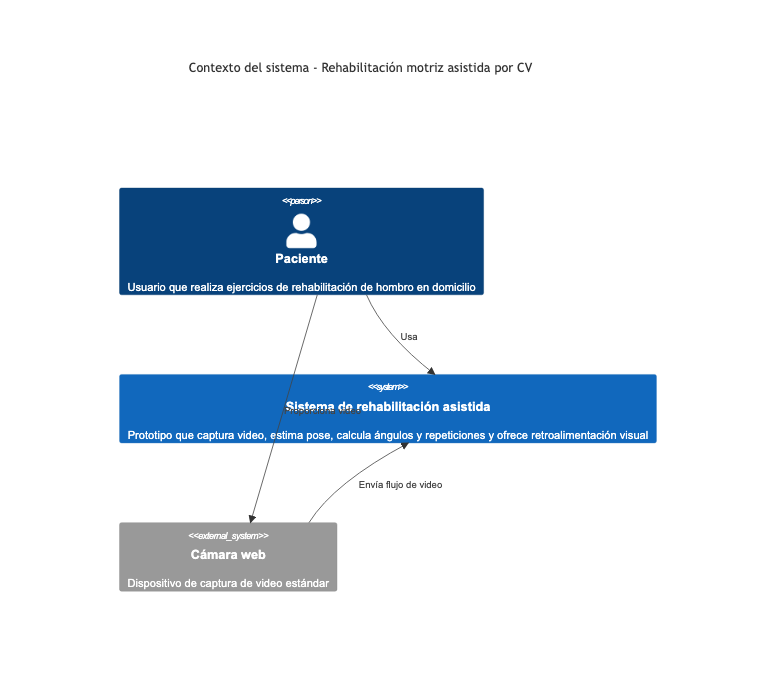
\includegraphics[width=0.85\linewidth,height=0.38\textheight,keepaspectratio]{arquitectura_c4_context.png}
\caption{Contexto del sistema (C4, nivel 1): usuario, sistema y cámara web.}
\label{fig:arquitectura-contexto}
\raggedright\footnotesize Fuente: Elaboración propia.
\end{figure}
\vspace{0.6em}
\begin{figure}[htbp]
\centering
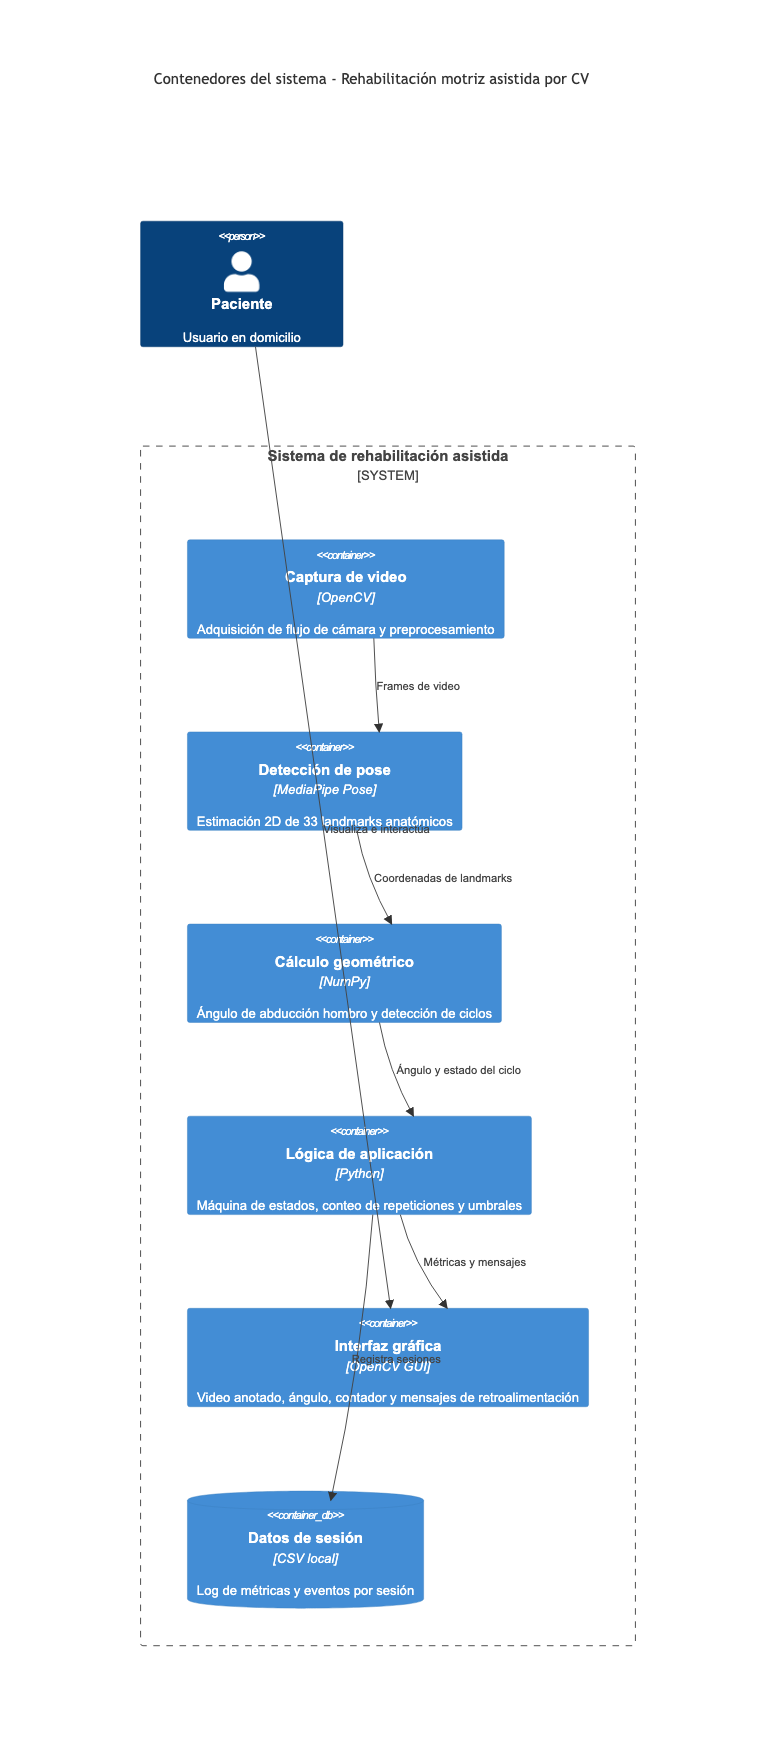
\includegraphics[width=0.9\linewidth,height=0.48\textheight,keepaspectratio]{arquitectura_c4_container.png}
\caption{Contenedores del sistema (C4, nivel 2): \mbox{pipeline} de captura, pose, cálculo, lógica, GUI y persistencia.}
\label{fig:arquitectura-contenedores}
\raggedright\footnotesize Fuente: Elaboración propia.
\end{figure}
\captionsetup[figure]{justification=justified,singlelinecheck=true}
\vspace{0.6em}
\noindent Como se observa en las Figuras~\ref{fig:arquitectura-contexto} y~\ref{fig:arquitectura-contenedores}, el sistema queda acotado al usuario, la cámara y el pipeline local hasta la persistencia en CSV.

\vspace{0.6em}
Componentes tecnológicos.
\begin{itemize}
  \item Lenguaje y entorno: Python 3.9+ con entornos virtuales (\texttt{venv}).
  \item IDE: Visual Studio Code.
  \item Librerías: OpenCV (captura, procesamiento, GUI); MediaPipe (estimación de pose 2D, modelo \texttt{pose\_landmarker\_lite.task} por defecto); NumPy (cálculos); Pandas y Matplotlib/Seaborn (análisis y gráficos).
  \item Gestión de datos: cada sesión genera un archivo CSV local con el esquema descrito en el \hyperref[anexo:csv-sesion]{Anexo~E} (\texttt{timestamp}, \texttt{frame\_id}, coordenadas normalizadas de hombro, codo y cadera, \texttt{angle\_deg}, \texttt{rep\_state}, \texttt{feedback\_msg}). Las coordenadas están en rango típico $[0,1]$ respecto al fotograma (pueden salir ligeramente fuera por el modelo de pose). No se almacenan videos crudos en el flujo estándar del MVP; el archivo de sesión no incluye nombre, contacto ni identificadores personales. La sensibilidad de estos datos es principalmente \textbf{cinemática y técnica}; no sustituye medidas clínicas identificadas. Cualquier archivo de video o imagen facial archivado para el estudio se trata aparte y exige las garantías del consentimiento informado (Anexo~A).
  \item Repositorio: Git en GitHub: \href{https://github.com/amc42357/master}{\texttt{github.com/amc42357/master}}; estructura \texttt{/src}, \texttt{/docs}, \texttt{/data}, \texttt{/tests}, README y \texttt{requirements.txt}.
\end{itemize}

\subsection{Despliegue (entorno, seguridad, contingencia)}
\textbf{Entorno de ejecución.} El prototipo se despliega como aplicación de escritorio en la máquina del usuario (Windows~10/11, macOS y, con las debidas pruebas, distribuciones Linux). La instalación reproduce el entorno mediante Python~3.9+ y un entorno virtual (\texttt{venv}) con dependencias fijadas en \texttt{requirements.txt}, de forma que la validación y las demos sean reproducibles. No se prevé, en el alcance del MVP, empaquetado instalador firmado ni distribución por tiendas de aplicaciones; un usuario avanzado clona el repositorio, activa el entorno y ejecuta el punto de entrada documentado en el README.

\textbf{Seguridad y privacidad.} El procesamiento de vídeo y la estimación de pose ocurren íntegramente en local: no se requiere conexión a Internet durante el uso rutinario ni se envían flujos de cámara a servicios externos. Los registros por sesión se escriben en CSV en disco bajo control del usuario (véase \hyperref[anexo:csv-sesion]{Anexo~E}); conviene ubicar la carpeta de datos en un volumen cifrado o con permisos restringidos si el equipo es compartido. Antes de sesiones de validación con grabación, se informa a los participantes según el Anexo~A. Las dependencias de terceros (OpenCV, MediaPipe, NumPy) deben mantenerse actualizadas ante avisos de seguridad del ecosistema Python.

\textbf{Contingencia y continuidad operativa.} El código se respalda mediante control de versiones (commits frecuentes, ramas por funcionalidad, remoto en GitHub). Si la detección de pose falla (iluminación extrema, oclusión, cámara desconectada), la interfaz debe degradarse de forma controlada: mensaje al usuario, posibilidad de reintentar la captura y registro del incidente en bitácora o en \texttt{KNOWN\_ISSUES.md}. Para pérdida de datos locales se recomienda copia de los CSV y del consentimiento fuera del equipo de prueba. Un plan mínimo de recuperación incluye: restaurar último tag estable, reinstalar dependencias desde \texttt{requirements.txt} y repetir una sesión de humo (captura + pose + exportación CSV).

\subsection{Mantenimiento (versionado, cambios y evolución)}
\textbf{Versionado del producto.} Las entregas etiquetadas siguen Versionado Semántico (SemVer: \texttt{MAJOR.MINOR.PATCH}): incremento mayor ante cambios incompatibles de API o flujo, menor ante nuevas funcionalidades retrocompatibles y parche ante correcciones. Cada release en GitHub se asocia a un tag y, cuando aplique, a notas breves de cambios (changelog en \texttt{CHANGELOG.md} o sección del README).

\textbf{Gestión de cambios en código.} Las modificaciones entran por ramas de corta duración y Pull Requests revisados por al menos otro miembro del equipo de desarrollo; el Product Owner valida el incremento en la Sprint Review según la DoD (Sección~4). No se fusiona a la rama principal código que rompa pruebas automatizadas o el flujo demo documentado. Los umbrales angulares, el modelo MediaPipe (\texttt{lite} vs \texttt{full}) y el formato CSV se tratan como contratos: un cambio que los altere exige actualizar README, Anexo~E y scripts de análisis en el mismo incremento.

\textbf{Mantenimiento evolutivo.} La base de código se estructura para facilitar nuevos ejercicios (otras articulaciones o reglas de conteo), mejoras de interfaz y, en fases posteriores, perfiles de usuario o historial. La dependencia de componentes de código abierto maduros reduce el riesgo de obsolescencia, pero impone revisiones periódicas de compatibilidad (versiones de Python, wheel de OpenCV/MediaPipe) y, si fuera necesario, congelación de dependencias para estudios longitudinales reproducibles.

\clearpage
\needspace{5\baselineskip}
\section{Validación y diseño experimental}

El diseño experimental evalúa el rendimiento del sistema mediante comparación con baseline (goniómetro, conteo humano), con métricas reproducibles.

\subsection{Hipótesis}
\begin{enumerate}
  \item H1: El sistema logrará medir el ángulo de abducción del hombro con MAE $\leq$ 5° frente a goniómetro.
  \item H2: El algoritmo de conteo alcanzará precisión $\geq$ 95\,\% respecto al conteo de un evaluador humano.
  \item H3: La latencia total (captura hasta retroalimentación en pantalla) será $<$ 150\,ms.
\end{enumerate}

\subsection{Métricas de evaluación}
Las métricas cuantitativas del experimento se definen de forma reproducible. El MAE (Error Absoluto Medio) del ángulo, con goniómetro como referencia, es
\begin{equation}
  \mathrm{MAE}_\theta = \frac{1}{N} \sum_{i=1}^{N} \bigl| \theta_{\mathrm{gonio},i} - \hat{\theta}_i \bigr|
\end{equation}
con $N$ repeticiones, $\theta_{\mathrm{gonio},i}$ ángulo medido con goniómetro y $\hat{\theta}_i$ ángulo del sistema. La precisión de conteo es
\begin{equation}
  P_{\mathrm{count}} = \frac{\#\,\text{repeticiones correctamente contadas}}{\#\,\text{repeticiones (referencia humano)}} \times 100\,\text{\%}\,.
\end{equation}
La latencia se mide como el tiempo entre el evento de movimiento (p. ej. paso por umbral angular) y la actualización correspondiente en pantalla. En la Tabla~\ref{tab:metricas} se resumen métricas, baselines y criterios: MAE $\leq$ 5°; precisión $\geq$ 95\,\%; latencia $<$ 150\,ms; robustez cualitativa (estabilidad en $\geq$ 3 condiciones de iluminación).

\begin{table}[htbp]
\caption{Resumen de métricas, baselines y criterios de éxito.}
\label{tab:metricas}
\small
\centering
\renewcommand{\arraystretch}{1.5}
\begin{tabular}{@{}p{2.6cm}p{3.4cm}p{3cm}p{2.6cm}@{}}
\toprule
Métrica & Definición & Baseline & Criterio \\
\midrule
Error angular (MAE) & Diferencia promedio absoluta sistema vs. referencia. & Goniómetro manual. & MAE $\leq$ 5° \\
\addlinespace
Precisión en conteo & \% repeticiones correctamente contadas. & Conteo visual por evaluador. & $\geq$ 95\,\% \\
\addlinespace
Latencia & Retraso evento--retroalimentación. & Cronómetro sobre video 60 FPS. & $<$ 150\,ms \\
\addlinespace
Robustez & Funcionamiento bajo variaciones. & Observación en pruebas. & Estable en $\geq$ 3 condiciones de luz. \\
\bottomrule
\end{tabular}\\
\renewcommand{\arraystretch}{1.35}
\vspace{4pt}
\raggedright\footnotesize Fuente: Elaboración propia (protocolo experimental).
\end{table}
\vspace{0.6em}

\subsection{Protocolo experimental}
Preparación: reclutamiento de 5 sujetos sanos adultos (muestreo por conveniencia), diestros, sin patología en hombro derecho; consentimiento informado (objetivo, participación, anonimato, procesamiento local, riesgos y beneficios). El tamaño $n=5$ se considera adecuado para prueba de concepto técnica (Debnath et al., 2021). Configuración: sujeto a 2\,m de cámara web (Logitech C920, 1080p, 30 FPS), iluminación uniforme, puntos anatómicos marcados, evaluador con goniómetro. Ejecución: 3 series de 10 repeticiones de abducción de hombro (ritmo metrónomo 1 rep/3\,s). Datos del sistema: registro CSV por sesión con el formato detallado en el \hyperref[anexo:csv-sesion]{Anexo~E} (incluye \texttt{angle\_deg}, \texttt{rep\_state} con valores \texttt{up}/\texttt{down} según la máquina de estados, y \texttt{feedback\_msg} cuando el sistema emite mensajes como \textit{Repetición válida}). Datos baseline: ángulo máximo por repetición con goniómetro; conteo de repeticiones válidas por evaluador. Análisis: sincronización por \texttt{timestamp}; scripts en Python (Pandas, SciPy) para MAE, precisión y latencia; gráficos de dispersión y series temporales. A título ilustrativo, una sesión de validación interna conservada en el repositorio (\texttt{rehab\_cv/data/}) puede abarcar del orden de $10^3$ filas y más de 100\,s de ejercicio continuo, según ritmo y FPS efectivos.

\subsection{Consideraciones normativas y éticas}
El protocolo de validación se alinea con el marco normativo y ético aplicable a la investigación con participantes humanos y al tratamiento de datos en el ámbito sanitario. En España, la Ley 14/2007, de 3 de julio, de Investigación biomédica, exige consentimiento informado expreso, información clara y comprensible, y derecho a revocación (BOE-A-2007-12945). La Ley 41/2002 básica de autonomía del paciente regula el derecho a la información y al consentimiento en el ámbito asistencial. El tratamiento de datos personales y de imágenes se ajusta al Reglamento (UE) 2016/679 (RGPD) y a la Ley Orgánica 3/2018 de protección de datos personales y garantía de los derechos digitales (LOPDGDD): minimización de datos, limitación de la finalidad (validación técnica), procesamiento local sin cesión a terceros. Los \textbf{CSV de sesión} (coordenadas normalizadas y ángulos) no contienen por diseño datos directamente identificativos; su tratamiento se orienta a la finalidad de validación técnica y reproducibilidad, sin confundir ``anonimización'' con el borrado de columnas técnicas necesarias para el análisis. En cambio, \textbf{grabaciones de vídeo o material facial} conservado más allá del procesamiento en vivo sí pueden ser datos personales sensibles y requieren las medidas acordadas en el consentimiento (p.\,ej. pseudonimización de ficheros, acceso restringido, plazo de conservación). La anonimización agresiva de datos cinemáticos no aporta beneficio privacy cuando no hay enlace a identidad en el conjunto de datos. En el ámbito de la Unión Europea, el Reglamento (UE) 2024/1689 por el que se establecen normas armonizadas en materia de inteligencia artificial (en vigor desde agosto de 2024) aplica un enfoque basado en el riesgo; el presente prototipo se enmarca en una fase de validación técnica con sujetos sanos, sin uso clínico ni diagnóstico, por lo que se sitúa en un contexto de riesgo limitado y se adoptan principios de transparencia, privacidad y supervisión humana en el diseño del experimento. El consentimiento informado utilizado en el estudio incorpora los elementos exigidos por la práctica habitual en investigación biomédica: objetivo del estudio, descripción de la participación, garantías de anonimato y procesamiento local, riesgos y beneficios, y declaración de consentimiento voluntario revocable.

\subsection{Resultados esperados y discusión}
\textbf{Rango esperado y comparativa.} Con sujetos sanos, iluminación uniforme y cámara a 2\,m, es razonable esperar un MAE angular en torno a 3°--5° respecto al goniómetro, coherente con el orden de magnitud reportado en la literatura para pose estimation en rehabilitación (p.\,ej. PoseRx con MAE $\approx$ 5,4°; Anexo~D) y con el criterio fijado para el MVP. La precisión de conteo debería situarse preferentemente entre 96\,\% y 100\,\% si los umbrales y la máquina de estados están alineados con el ritmo metronómico del protocolo. La latencia end-to-end en equipos de gama media suele permanecer por debajo de 100\,ms cuando el pipeline no está saturado, cumpliendo holgadamente el umbral de 150\,ms definido como hipótesis H3.

\textbf{Errores y fuentes de discrepancia.} Las principales fuentes de error angular son: (1) \textit{paralaje} entre la línea de visión de la cámara y el plano de movimiento del brazo; (2) \textit{oclusiones} parciales o pérdida temporal de landmarks; (3) \textit{discretización temporal} (FPS efectivos y suavizado) que desplaza el instante del máximo angular respecto al instante muestreado con goniómetro; (4) \textit{variabilidad intra- e inter-sujeto} en la ejecución del arco de movimiento. En el conteo, los fallos suelen deberse a umbrales demasiado estrictos o laxos, a repeticiones incompletas contadas como válidas y a feedback textual que no coincide con el estado interno (\texttt{rep\_state}). El análisis debe desagregar MAE por serie y por sujeto, y cruzar picos de \texttt{angle\_deg} con lecturas de goniómetro sincronizadas por \texttt{timestamp}.

\textbf{Implicaciones.} Un cumplimiento de los criterios MAE $\leq$ 5° y precisión $\geq$ 95\,\% \textbf{no} implica eficacia clínica ni seguridad terapéutica: solo respalda la \textbf{validez técnica} del prototipo en el ejercicio y población de prueba descritos. Una desviación sistemática por encima del umbral indicaría necesidad de recalibración (geometría, modelo MediaPipe, reglas de conteo) antes de cualquier extensión a pacientes reales. Los hallazgos de Unger et al.\ (2025) sobre generalización interindividual refuerzan que un siguiente paso lógico sería personalización o adaptación leve por sujeto, fuera del alcance del MVP actual.

\clearpage
\needspace{5\baselineskip}
\section{Conclusiones y trabajo futuro}

\subsection{Conclusiones}
El trabajo ha diseñado y planificado un sistema de asistencia para rehabilitación motriz domiciliaria post-ACV basado en visión por computadora, que responde al reto de diseño con un enfoque centrado en accesibilidad, viabilidad técnica y privacidad.

La aplicación de Design Thinking permitió anclar la solución en las necesidades de pacientes y terapeutas y en la brecha de supervisión objetiva en el hogar. El estado del arte mostró un hueco para una solución práctica y escalable que combine software de IA de código abierto con hardware de consumo. Scrum y Lean Startup estructuran un plan de ejecución realista en 16 semanas, con entregas incrementales y un MVP bien acotado. El diseño experimental aporta hipótesis comprobables, métricas objetivas (MAE $\leq$ 5°, precisión $\geq$ 95\,\%) y baseline con goniómetro.

En relación con los objetivos: el objetivo general se cumple mediante el prototipo descrito y su validación frente a goniómetro y conteo humano; los objetivos específicos 1 a 3 se materializan en el código y la GUI (módulo de pose, análisis cinemático, interfaz con retroalimentación); el objetivo 4 en el protocolo de la Sección 6 y los resultados de las pruebas; el objetivo 5 en el repositorio con README, código documentado e informe de validación.

\subsection{Limitaciones y trabajo futuro}
Limitaciones: (1) validación con población simulada (sujetos sanos); (2) alcance clínico reducido (un solo ejercicio); (3) entorno controlado. Trabajo futuro: (1) estudio piloto con pacientes reales post-ACV ($n=5$--10); (2) ampliación de la biblioteca de ejercicios (codo, escapular, rodilla, tobillo); (3) personalización y entrenamiento adaptativo; (4) integración con historial clínico electrónico (estándares FHIR); (5) investigación de robustez con transfer learning para movimientos atípicos.

El proyecto sirve de punto de partida para abordar un problema de salud complejo con un enfoque pragmático y centrado en el usuario.

\clearpage
% ========== 8. ANEXOS ==========
\section*{Anexos}
\addcontentsline{toc}{section}{Anexos}
\label{sec:anexos}

\subsection*{Anexo A. Consentimiento informado (resumen)}
El protocolo de validación (Sección 6) contempla la obtención de consentimiento informado firmado por cada participante. El documento incluye: objetivo del estudio (validación técnica del sistema de visión por computadora para rehabilitación), descripción de la participación (incluida, si aplica, grabación en video para análisis técnico), garantías de anonimato y procesamiento local de imágenes, riesgos y beneficios, y declaración de consentimiento voluntario. Se informa asimismo de la generación de \textbf{registros CSV} con datos cinemáticos agregados por fotograma (véase \hyperref[anexo:csv-sesion]{Anexo~E}), distintos de la identidad del participante. El texto completo del consentimiento se encuentra en los materiales del proyecto (repositorio y carpeta de documentación del seminario).

\subsection*{Anexo B. Evidencia de gestión en Jira}
\label{anexo:jira}
Evidencia de la instancia Jira local utilizada para el seguimiento del proyecto: backlog del producto (épicas E1--E3 e historias US-01 a US-10, tareas T-07 a T-09) y board del sprint activo (columnas Por hacer / En progreso / Hecho). Como se muestra en las Figuras~\ref{fig:jira-backlog} y~\ref{fig:jira-board}, el backlog y el board de sprint reflejan el estado de las historias y tareas descritas en la Sección~4. Las capturas se generan desde el repositorio con los scripts en \texttt{scripts/} (inyección de datos, asignación a sprint y captura de pantalla).

\vspace{1em}
\IfFileExists{docs/evidencias_jira/jira_board_backlog.png}{%
\begin{figure}[htbp]
\centering
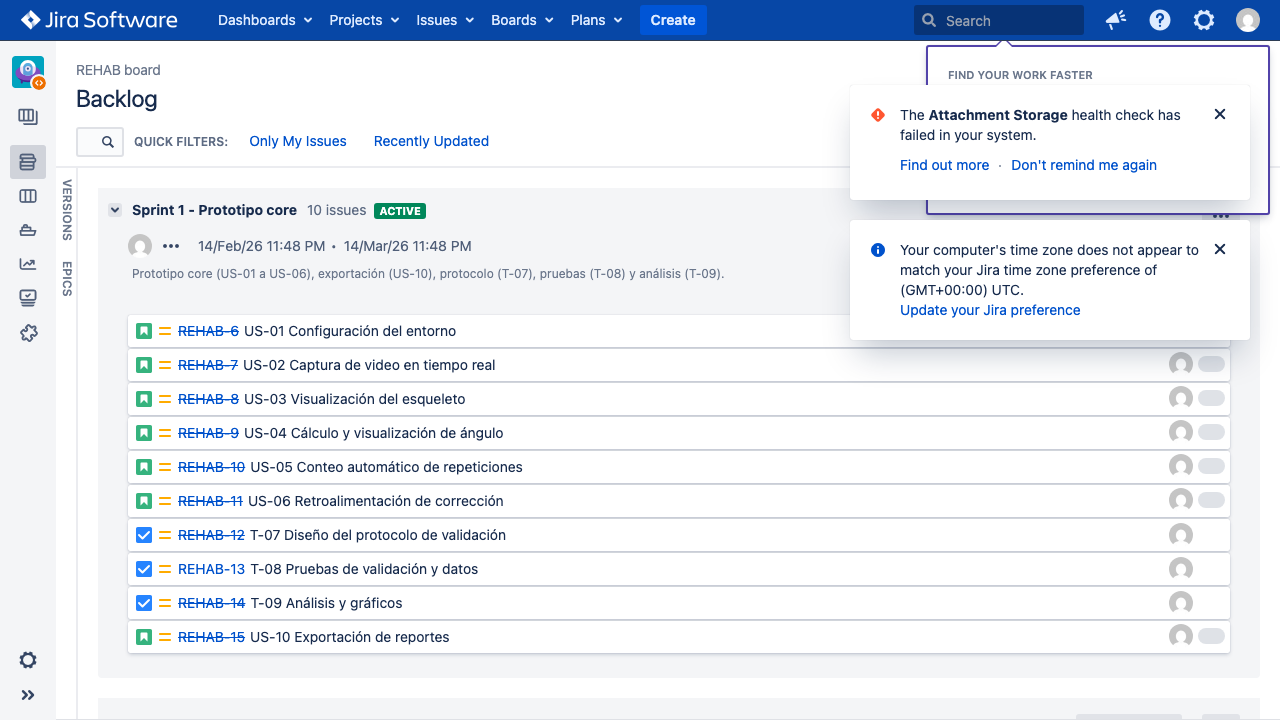
\includegraphics[width=0.9\linewidth,height=0.42\textheight,keepaspectratio]{docs/evidencias_jira/jira_board_backlog.png}
\caption{Backlog del producto en Jira (épicas e historias).}
\label{fig:jira-backlog}
\raggedright\footnotesize Fuente: Captura de pantalla del proyecto en Jira. Elaboración propia.
\end{figure}
\vspace{0.8em}
}{%
\noindent [Figura: Backlog del producto en Jira. Añadir \texttt{jira\_board\_backlog.png} en \texttt{docs/evidencias\_jira/}.]
\label{fig:jira-backlog}
\par\vspace{0.6em}
}%
\IfFileExists{docs/evidencias_jira/jira_board_sprint.png}{%
\begin{figure}[htbp]
\centering
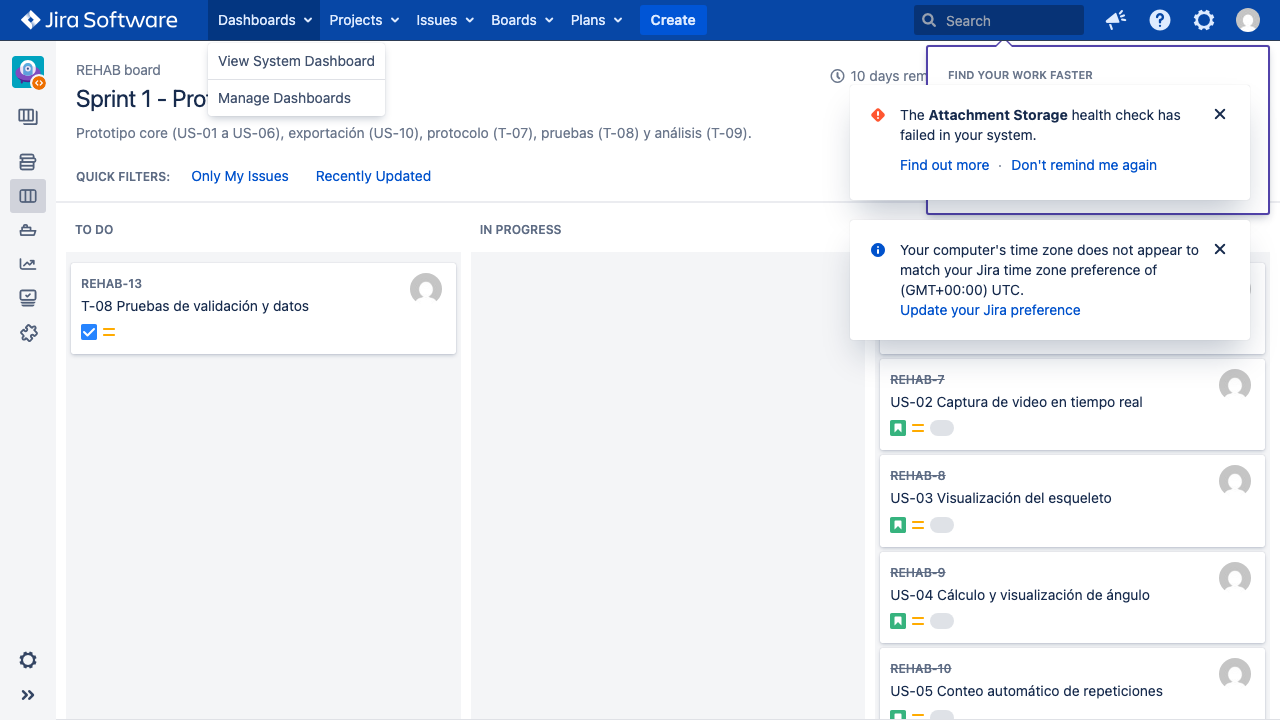
\includegraphics[width=0.9\linewidth,height=0.42\textheight,keepaspectratio]{docs/evidencias_jira/jira_board_sprint.png}
\caption{Board de sprint en Jira (columnas Por hacer / En progreso / Hecho).}
\label{fig:jira-board}
\raggedright\footnotesize Fuente: Captura de pantalla del proyecto en Jira. Elaboración propia.
\end{figure}
}{%
\noindent [Figura: Board de sprint en Jira. Añadir \texttt{jira\_board\_sprint.png} en \texttt{docs/evidencias\_jira/}.]
\label{fig:jira-board}
\par\vspace{0.6em}
}%

\subsection*{Anexo C. Empatía: decisión sobre fuente primaria local}
\label{anexo:fuente-primaria}
La etapa Empatizar (Sección~3.1) se sustenta en \textbf{datos primarios ya publicados}: el estudio de factibilidad con participantes post-ictus de Unger et al.\ (2025), analizado en el cuerpo del documento y sintetizado en la Tabla~\ref{tab:empatizar}, complementado con revisión bibliográfica y criterios clínicos de referencia. Para el calendario del seminario y el alcance de esta entrega, \textbf{no se realizó entrevista ni observación local adicional} con terapeutas o pacientes; se consideró que la triangulación con Unger et al.\ y la literatura secundaria ofrece base suficiente para formular el reto HMW y los criterios de éxito del MVP.

Este anexo deja constancia de esa decisión y ofrece una \textbf{plantilla reutilizable} si en iteraciones futuras se incorpora fuente primaria local (p.\,ej. validación con profesionales o observación de sesión domiciliaria simulada):

\begin{itemize}
  \item \textbf{Fecha y modalidad:} registro de la sesión (entrevista semiestructurada u observación estructurada) y canal (presencial, videollamada).
  \item \textbf{Perfil del informante o contexto:} rol (fisioterapeuta, médico rehabilitador, cuidador), años de experiencia o relación con el paciente; en observación, descripción breve del entorno y del ejercicio supervisado.
  \item \textbf{Instrumento:} guion de entrevista o ficha de observación (preguntas abiertas sobre barreras de adherencia, necesidad de métricas objetivas y privacidad); ubicación del archivo en el repositorio bajo \texttt{/docs}.
  \item \textbf{Síntesis:} dos o tres hallazgos textuales que maticen o refuercen filas de la Tabla~\ref{tab:empatizar}, con citas o transcripción anonimizada según consentimiento.
\end{itemize}

Así, el Anexo~C queda cerrado para la versión actual del documento, sin campos pendientes, y alineado con la trazabilidad Design Thinking descrita en la Sección~3.

\subsection*{Anexo D. Desglose de métricas y limitaciones (estimación de pose en rehabilitación)}
\label{anexo:estado-arte}
Este anexo complementa la Tabla~\ref{tab:estadoarte} con un estudio reciente centrado en pose estimation aplicada a rehabilitación (Shukla \& Rathore, 2025).

\begin{table}[htbp]
\caption{Estado del arte focalizado: PoseRx frente al posicionamiento del MVP (MediaPipe).}
\label{tab:anexo-pose}
\footnotesize
\centering
\renewcommand{\arraystretch}{1.25}
\begin{tabular}{@{}p{2.1cm}p{2.35cm}p{2.5cm}p{2.35cm}p{2.55cm}@{}}
\toprule
Estudio & Tecnología / modelo & Métricas reportadas & Limitaciones & Posicionamiento frente a esta propuesta \\
\midrule
Shukla y Rathore (2025) & PoseRx (TokenPose / transformador) para rehabilitación. & MAE angular 5,4°; error de localización 2D 5,9 px; alta robustez ante oclusiones. & Arquitectura de transformador más compleja que una solución basada en MediaPipe; enfoque de investigación, menos directo para un MVP ligero. & Esta propuesta usa MediaPipe en hardware de consumo. El MAE de 5,4° en PoseRx actúa como baseline para justificar el criterio MAE $\leq$ 5° del MVP. \\
\bottomrule
\end{tabular}\\
\renewcommand{\arraystretch}{1.35}
\vspace{4pt}
\raggedright\footnotesize Fuente: Shukla y Rathore (2025).
\end{table}
\vspace{0.5em}

\subsection*{Anexo E. Formato del registro CSV de sesión (US-10)}
\label{anexo:csv-sesion}
El prototipo exporta un archivo \texttt{.csv} por sesión (UTF-8, separador coma), generado por el módulo \texttt{session\_logger} del repositorio. La primera fila es cabecera; cada fila siguiente corresponde a un fotograma o instante de registro. La Tabla~\ref{tab:csv-columnas} resume los campos.

\begin{table}[htbp]
\caption{Campos del CSV de sesión.}
\label{tab:csv-columnas}
\footnotesize
\centering
\renewcommand{\arraystretch}{1.2}
\begin{tabular}{@{}p{2.6cm}p{9.8cm}@{}}
\toprule
Campo & Descripción \\
\midrule
\texttt{timestamp} & Segundos transcurridos desde el inicio del registro de la sesión (resolución milisegundos en el fichero). \\
\texttt{frame\_id} & Índice entero monótono del fotograma (0, 1, 2, \ldots). \\
\texttt{shoulder\_x}, \texttt{shoulder\_y} & Coordenadas normalizadas del landmark hombro en imagen. \\
\texttt{elbow\_x}, \texttt{elbow\_y} & Coordenadas normalizadas del landmark codo. \\
\texttt{hip\_x}, \texttt{hip\_y} & Coordenadas normalizadas del landmark cadera. \\
\texttt{angle\_deg} & Ángulo de abducción estimado en grados (una decimal en exportación). \\
\texttt{rep\_state} & Estado de la máquina de estados del conteo: \texttt{up} (fase ascendente del movimiento) o \texttt{down} (fase descendente o reposo según la lógica implementada). \\
\texttt{feedback\_msg} & Texto de retroalimentación en ese instante; vacío si no hay mensaje. Incluye, entre otros, la cadena \textit{Repetición válida} cuando el sistema confirma un ciclo completo. \\
\bottomrule
\end{tabular}\\
\renewcommand{\arraystretch}{1.35}
\vspace{4pt}
\raggedright\footnotesize Fuente: implementación en \texttt{rehab\_cv/src/session\_logger.py}. Elaboración propia.
\end{table}

\vspace{0.5em}
\noindent\textbf{Ejemplo sintético} (tres filas; valores ilustrativos). En el fichero real la cabecera es una sola línea; aquí se parte solo por limitaciones de ancho en PDF:

{\footnotesize
\begin{verbatim}
timestamp,frame_id,shoulder_x,shoulder_y,elbow_x,elbow_y,
hip_x,hip_y,angle_deg,rep_state,feedback_msg
0.000,0,0.4500,0.2900,0.4000,0.5100,0.4750,0.7750,16.1,down,
1.027,15,0.4538,0.2995,0.4024,0.5662,0.4858,0.8299,14.4,down,
8.257,151,0.4674,0.3571,0.3705,0.4183,0.4852,0.7390,60.4,up,
\end{verbatim}
}

\noindent Estas cifras son coherentes con sesiones reales de prueba (variación angular durante el ciclo, alternancia \texttt{down}/\texttt{up}). Para análisis cuantitativos del MVP se utilizan los ficheros bajo \texttt{rehab\_cv/data/} (p.\,ej.\ sesiones de $\sim$100--1600 filas según duración).

\clearpage
% ========== 9. REFERENCIAS ==========
\section*{Referencias}
\addcontentsline{toc}{section}{Referencias}

\noindent American Psychological Association. (2020). \textit{Publication manual of the American Psychological Association} (7.ª ed.).

\noindent Basteris, A., Nijenhuis, S. M., Stienen, A. H., Buurke, J. H., Prange, G. B., \& Amirabdollahian, F. (2014). Training modalities in robot-mediated upper limb rehabilitation in stroke: A framework for classification based on a systematic review. \textit{Journal of NeuroEngineering and Rehabilitation}, \textit{11}(1), 111. \url{https://doi.org/10.1186/1743-0003-11-111}

\noindent Debnath, B., O'Brien, M., Yamaguchi, M., \& Behera, A. (2021). A review of computer vision-based approaches for physical rehabilitation and assessment. \textit{Multimedia Systems}, \textit{28}, 209--239. \url{https://doi.org/10.1007/s00530-021-00815-4}

\noindent Esteva, A., Robicquet, A., Ramsundar, B., Kuleshov, V., DePristo, M., Chou, K., Cui, C., Corrado, G., Thrun, S., \& Dean, J. (2019). A guide to deep learning in healthcare. \textit{Nature Medicine}, \textit{25}(1), 24--29. \url{https://doi.org/10.1038/s41591-018-0316-z}

\noindent Instituto Nacional de Estadística y Geografía. (2021). \textit{Estadísticas de defunciones registradas 2020}. \url{https://www.inegi.org.mx/contenidos/saladeprensa/boletines/2021/EstSociodemo/DefuncionesRegistradas2020_Pnles.pdf}

\noindent Langhorne, P., Bernhardt, J., \& Kwakkel, G. (2011). Stroke rehabilitation. \textit{The Lancet}, \textit{377}(9778), 1693--1702. \url{https://doi.org/10.1016/S0140-6736(11)60325-5}

\noindent Laver, K. E., Adey-Wakeling, Z., Crotty, M., Lannin, N. A., George, S., \& Sherrington, C. (2020). Telerehabilitation services for stroke. \textit{Cochrane Database of Systematic Reviews}, \textit{2020}(1), CD010255. \url{https://doi.org/10.1002/14651858.CD010255.pub3}

\noindent National Institute of Neurological Disorders and Stroke. (2020). \textit{Post-stroke rehabilitation}. National Institutes of Health. \url{https://www.ninds.nih.gov/health-information/stroke/recovery}

\noindent Organización Mundial de la Salud. (2017). \textit{Rehabilitation in health systems}. \url{https://iris.who.int/handle/10665/254506}

\noindent Ries, E. (2011). \textit{The Lean Startup: How today's entrepreneurs use continuous innovation to create radically successful businesses}. Crown Currency.

\noindent Saposnik, G., Cohen, L. G., Mamdani, M., Pooyania, S., Ploughman, M., Cheung, D., Shaw, J., Hall, J., Nord, P., Dukelow, S., Nilanont, Y., De Los Rios, F., Olmos, L., Levin, M., Teasell, R., Cohen, A., Thorpe, K., Laupacis, A., \& Bayley, M. (2016). Efficacy and safety of non-immersive virtual reality exercising in stroke rehabilitation (EVREST): A randomised, multicentre, single-blind, controlled trial. \textit{The Lancet Neurology}, \textit{15}(10), 1019--1027. \url{https://doi.org/10.1016/S1474-4422(16)30121-1}

\noindent Shukla, D., \& Rathore, M. (2025). PoseRx: A transformer-based remedy for precision in physical rehabilitation monitoring. \textit{Journal of Information Systems Engineering and Management}, \textit{10}(37s). \url{https://doi.org/10.52783/jisem.v10i37s.6733}

\noindent Unger, T., K\"uhnis, B., Sauerzopf, L., Spiess, M. R., de Spindler, A., Luft, A. R., Easthope Awai, C., Sch\"onhammer, J. G., \& Gavagnin, E. (2025). Using deep learning to detect upper limb compensation in individuals post-stroke using consumer-grade webcams---A feasibility study. \textit{Frontiers in Medicine}, \textit{12}, Article 1645369. \url{https://doi.org/10.3389/fmed.2025.1645369}

\vspace{0.5em}
\noindent Ley 14/2007, de 3 de julio, de Investigación biomédica. \textit{Boletín Oficial del Estado}, 159, 28826--28848. \url{https://www.boe.es/buscar/act.php?id=BOE-A-2007-12945}

\noindent Ley 41/2002, de 14 de noviembre, básica reguladora de la autonomía del paciente y de derechos y obligaciones en materia de información y documentación clínica. \textit{Boletín Oficial del Estado}, 274, 40126--40132.

\noindent Ley Orgánica 3/2018, de 5 de diciembre, de Protección de Datos Personales y garantía de los derechos digitales. \textit{Boletín Oficial del Estado}, 294, 119788--119857.

\noindent Parlamento Europeo y Consejo de la Unión Europea. (2016). Reglamento (UE) 2016/679 relativo a la protección de las personas físicas (RGPD). \textit{Diario Oficial de la Unión Europea}, L 119, 1--88.

\noindent Parlamento Europeo y Consejo de la Unión Europea. (2024). Reglamento (UE) 2024/1689 por el que se establecen normas armonizadas en materia de inteligencia artificial. \textit{Diario Oficial de la Unión Europea}, L 1689. \url{https://eur-lex.europa.eu/legal-content/ES/TXT/?uri=CELEX:32024R1689}

\end{document}
